\documentclass{article}

\usepackage{hyperref,graphicx,amsfonts}

\title{Lab 1 - Setup and Data Loading}
\author{Kyle Swanson}
\date{January 8, 2018}

\setcounter{section}{-1}

\begin{document}

\maketitle

\section{Introduction}

This lab will primarily consist of all the necessary setup for future labs. All labs in this class will be written in Python 3. Some labs will involve building machine learning algorithms from scratch in Python, while others will involve using pre-built Python machine learning packages. After you've finished all the setup steps, we'll use the rest of the time today to get used to working with data in Python.

\section{Lab Setup}

\subsection{GitHub}

All the materials in this class will be provided on the class GitHub: \url{https://github.com/swansonk14/IntroML}. The IntroML repository will be updated each day to include that day's lecture and lab material.

\begin{enumerate}
	\item If you do not have a GitHub account already, set one up here: \url{https://github.com/}.
	\item Log into \texttt{github.com} and create a new repository called ``\texttt{IntroML}". Instructions for creating a GitHub repo can be found here: \url{https://help.github.com/articles/create-a-repo/}.
	\item Clone the repo to your laptop. Instructions for cloning a repository can be found here: \url{https://help.github.com/articles/cloning-a-repository/}.
	\item Open a terminal, navigate to the repo, and perform the following command:

	\texttt{git remote add class https://github.com/swansonk14/IntroML.git}

	From now on, you can get the latest class material with:

	\texttt{git pull class master}

	After working on each lab, add all the files you modified with:

	\texttt{git add <filename>}

	Then, commit the changes using:

	\texttt{git commit -m "<Commit message>"}

	Finally, push the changes to your personal repo with:

	\texttt{git push origin master}

	If you're unfamiliar with git, please don't hesitate to ask me for help.
\end{enumerate}

\subsection{Python}

In this class we will be using Python 3. I recommend installing Python 3 with Anaconda. Anaconda is a Python distribution which includes many useful Python packages, some of which we will be using in this class. To download Anaconda, follow the steps on the relevant page:

\begin{itemize}
	\item Linux: \url{https://conda.io/docs/user-guide/install/linux.html}
	\item Mac: \url{https://conda.io/docs/user-guide/install/macos.html}
	\item Windows: \url{https://conda.io/docs/user-guide/install/windows.html}
\end{itemize}

Make sure to install Anaconda, \textit{not} Miniconda, since Anaconda includes all the packages we want whereas Miniconda doesn't.

If you don't want to use Anaconda, you may install Python directly from \url{https://www.python.org/downloads/}

\subsection{Python Packages}

In addition to Python, we need to install some relevant Python packages. If you installed Python with Anaconda, you only need to install \texttt{keras}. If you installed Python without Anaconda, you need to install all of the following packages. Packages can be installed with the Python Package Index (\url{https://pypi.python.org/pypi/pip}) by running

\vspace{2mm}
\texttt{pip install <package-name>}
\vspace{2mm}

\noindent
where \texttt{<package-name>} is replaced with each of the following package names:

\begin{itemize}
	\item \texttt{numpy} - Array processing
	\item \texttt{scipy} - Scientific computing
	\item \texttt{scikit-learn} - Machine learning
	\item \texttt{pillow} - Image processing
	\item \texttt{matplotlib} - Plotting
	\item \texttt{keras} - Deep learning
\end{itemize}

You can test these installations by opening a Python shell (just run the command \texttt{python} in the terminal) and then running \texttt{import <package-name>}. Note that to import \texttt{scikit-learn}, you should run the command \texttt{import sklearn}, and to import pillow, you should run \texttt{import PIL}. All other import names are the same as the package names.

\section{Data Loading and Plotting}

This final section is intended to give you some practice working with data in Python. If you don't have time to complete this section, don't worry about it -- I'll post solutions tomorrow.

\subsection{Data Loading}

In order to apply machine learning algorithms to our data, we need to load the data into Python in a form that makes sense for the problem we're trying to solve. One common data format is the Comma Separate Value (CSV) file. Data stored in spreadsheets (ex. Excel) can easily be converted to CSV format, so it's worth knowing how to load CSV files into Python.

To practice, we'll be loading a CSV file containing reviews of Amazon products. We'll run some machine learning algorithms on these reviews later in the week. All data in this class, including the Amazon reviews, can be found in the \texttt{Data} directory. Navigate to the \texttt{Data} directory and open up \texttt{reviews\_train.csv} in a text editor to see the format you will have to process.

Now navigate to \texttt{Labs/Lab1}. In the \texttt{Lab1} directory, you'll see two Python scripts, \texttt{main.py} and \texttt{lab1.py}. \texttt{main.py} is the script you will run, and it imports functions from \texttt{lab1.py} which you need to implement. For this part of the lab, the function you need to implement is \texttt{load\_reviews\_data}. Read the function specification in \texttt{lab1.py} and implement the function. I recommend using the Python csv module: \url{https://docs.python.org/3/library/csv.html}. (Hint: Look up the \texttt{DictReader} csv function.)

Once your implementation is complete, run \texttt{python main.py}. If you see

\vspace{2mm}
\texttt{Reviews data loaded correctly}
\vspace{2mm}

\noindent
printed to the terminal, then you have correctly implemented the function. Ignore any errors which may appear afterwards -- those will be fixed when you implement the remaining functions.

\subsection{Plotting}

Another useful skill when working with data is the ability to visualize data and results. Visualizing data is incredibly important when trying to determine what machine learning methods are appropriate for the dataset. Visualizing results can help you understand what your machine learning model is doing well and where it can be improved.

We'll practice this skill with a very simple example: plotting two-dimensional data points. The data we'll be working with is in \texttt{toy\_data.csv} in the \texttt{Data} directory. Open up the file with a text editor to see the format of the data. You'll see that the file consists of ``labels'', which are either $+1$ or $-1$, and $x$ and $y$ coordinates of data points.

 Your job is to implement two functions in \texttt{lab1.py}: \texttt{load\_toy\_data} and \texttt{plot\_toy\_data}.

 The function \texttt{load\_toy\_data} loads the text file and creates two arrays, a \texttt{data} array containing the two-dimensional points, and a \texttt{labels} array containing the label of the data point. To load this data, you can use the Python csv reader again if you'd like, but I found it easier to use the Numpy function \texttt{loadtxt} with \texttt{unpack = true} (\url{https://docs.scipy.org/doc/numpy-1.13.0/reference/generated/numpy.loadtxt.html}).

 The function \texttt{plot\_toy\_data} should take these two arrays and plot the data as a scatterplot with the $+1$ points in blue and the $-1$ points in red. Plotting in Python is typically done using Matplotlib. To create a scatterplot, take a look at the \texttt{scatter} function of \texttt{matplotlib.pyplot.scatter} (\url{https://matplotlib.org/devdocs/api/_as_gen/matplotlib.pyplot.scatter.html}). Note that \texttt{matplotlib.pyplot} has already been imported for you as \texttt{plt}, so you can call the \texttt{scatter} function with \texttt{plt.scatter()}.

Once your implementation is complete, run \texttt{python main.py}. There should be no errors, and you should see

\vspace{2mm}
\texttt{Reviews data loaded correctly}

\texttt{Toy data loaded correctly}
\vspace{2mm}

Additionally, you should see a new window open up with the toy data plot. Your plot should look like this:

\vspace{5mm}
\noindent
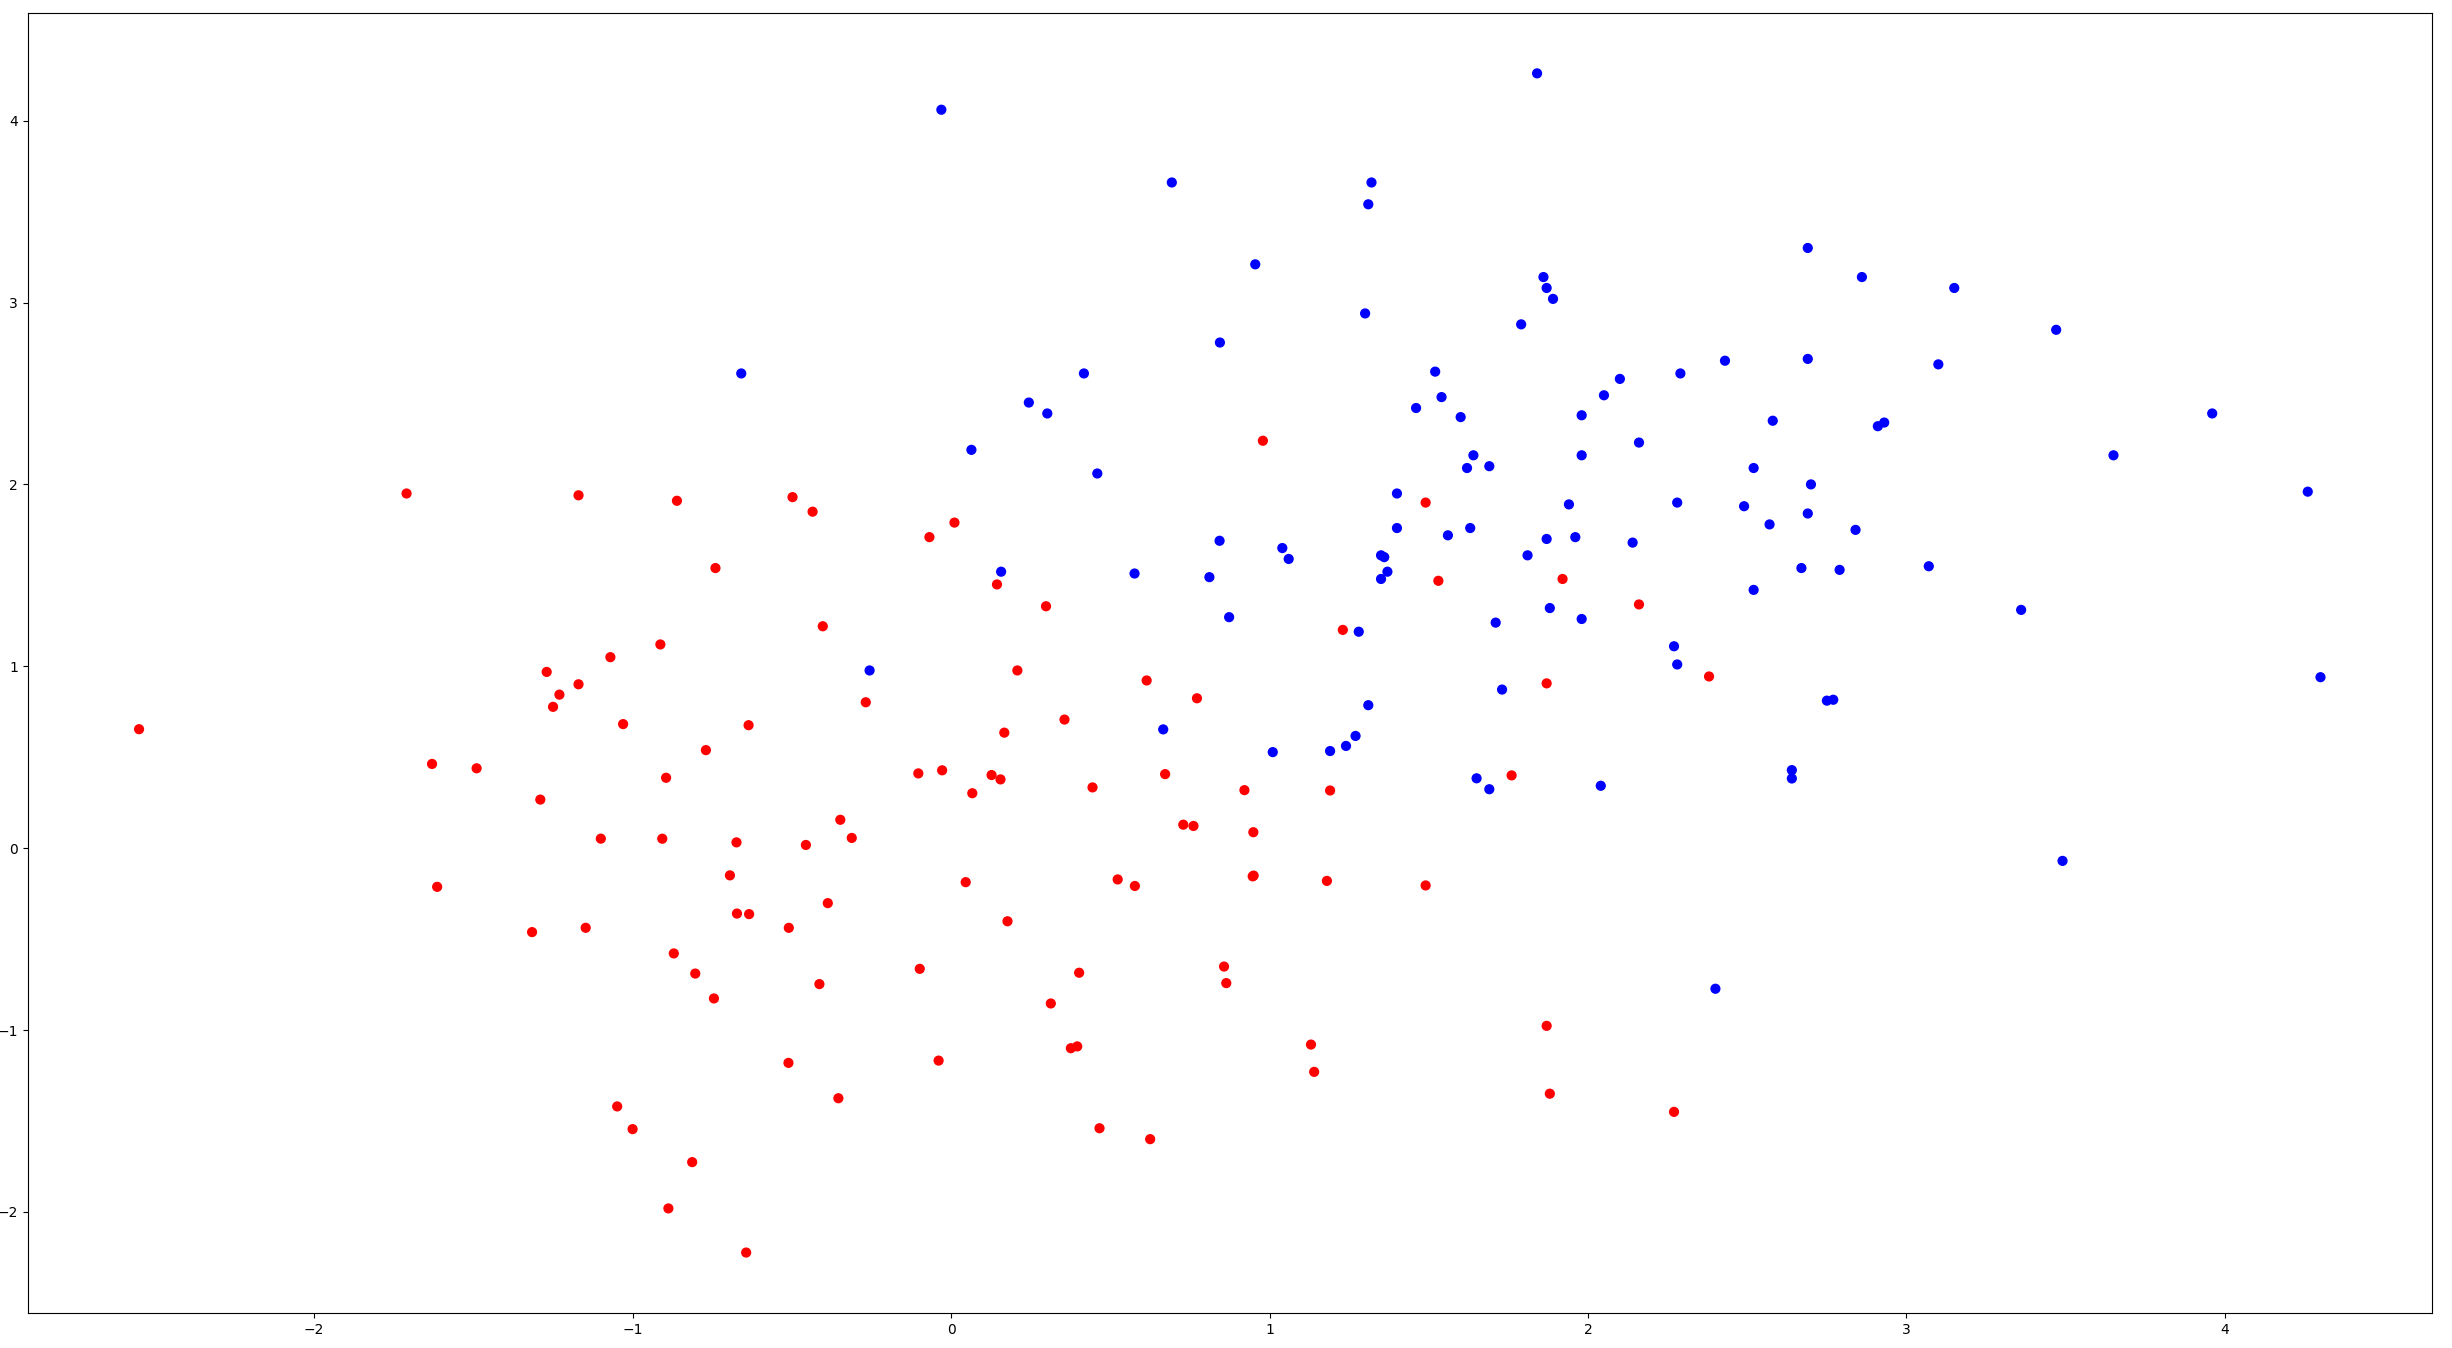
\includegraphics[width=\textwidth]{toy_data.png}
\vspace{5mm}

If your functions and plot are correct, you are done! Tomorrow we'll implement our first machine learning algorithm, the perceptron algorithm.

\subsection{Challenge: Plotting a Linear Decision Boundary}

This section is an extra challenge if you have time. In lecture today we talked about classifiers and decision boundaries. If you remember, a linear decision boundary is a line in $\mathbb{R}^2$ which divides the data points, so that on one side of the decision boundary we prediction positive (blue) and one the other side we predict negative (red).

First, try to guess a linear decision boundary for the data. Is it possible to perfectly separate the data? If not, what linear decision boundary would be best? Try to write an equation of the line for the decision boundary (write it in the form $y=ax+b$ where $a$ and $b$ are real numbers which you must choose).

Now, try plotting that line using \texttt{matplotlib} and \texttt{pyplot}. Google is your friend here. Try looking up how to plot lines using \texttt{pyplot} and you should find resources which will help. Let me know if you're having trouble.

Once you have plotted your best guess at the decision boundary, save the image. Tomorrow in lab we'll program a machine learning algorithm which will generate a linear decision boundary and you can compare your guess to the prediction of the algorithm.

\end{document}